%package list
\documentclass{article}
\usepackage[top=3cm, bottom=3cm, outer=3cm, inner=3cm]{geometry}
\usepackage{multicol}
\usepackage{graphicx}
\usepackage{url}
%\usepackage{cite}
\usepackage{hyperref}
\usepackage{array}
\usepackage{bookmark}
%\usepackage{multicol}
\newcolumntype{x}[1]{>{\centering\arraybackslash\hspace{0pt}}p{#1}}
\usepackage{natbib}
\usepackage{pdfpages}
\usepackage{multirow}
\usepackage[normalem]{ulem}
\useunder{\uline}{\ul}{}
\usepackage{xcolor}

%\usepackage{booktabs}
\usepackage[labelformat=empty]{caption}
\usepackage{subcaption}
\usepackage{float}
\usepackage{array}
\usepackage{minted}

\setminted{fontsize=\small,numbers=left,autogobble}
\newenvironment{block}{\captionsetup{type=listing}}{}

\newcolumntype{M}[1]{>{\centering\arraybackslash}m{#1}}
\newcolumntype{N}{@{}m{0pt}@{}}

% para el codigo fuente
\usepackage{listings}
\usepackage{color, colortbl}
\definecolor{dkgreen}{rgb}{0,0.6,0}
\definecolor{gray}{rgb}{0.5,0.5,0.5}
\definecolor{mauve}{rgb}{0.58,0,0.82}
\definecolor{codebackground}{rgb}{0.95, 0.95, 0.92}
\definecolor{tablebackground}{rgb}{0.8, 0, 0}

\lstset{frame=tb,
	language=bash,
	aboveskip=3mm,
	belowskip=3mm,
	showstringspaces=false,
	columns=flexible,
	basicstyle={\small\ttfamily},
	numbers=none,
	numberstyle=\tiny\color{gray},
	keywordstyle=\color{blue},
	commentstyle=\color{dkgreen},
	stringstyle=\color{mauve},
	breaklines=true,
	breakatwhitespace=true,
	tabsize=3,
	backgroundcolor= \color{codebackground},
}

%Comando
\newcommand{\itemEmail}{mjarama@unsa.edu.pe}
\newcommand{\itemStudent}{Mariel Alisson Jara Mamani}
\newcommand{\itemStudentShort}{Mariel Jara}
\newcommand{\itemCourse}{Programación Web 2}
\newcommand{\itemCourseCode}{1702122}
\newcommand{\itemSemester}{I}
\newcommand{\itemUniversity}{Universidad Nacional de San Agustín de Arequipa}
\newcommand{\itemFaculty}{Facultad de Ingeniería de Producción y Servicios}
\newcommand{\itemDepartment}{Departamento Académico de Ingeniería de Sistemas e Informática}
\newcommand{\itemSchool}{Escuela Profesional de Ingeniería de Sistemas}
\newcommand{\itemAcademic}{2023 \- B}
\newcommand{\itemInput}{Del 27 Mayo 2024}
\newcommand{\itemOutput}{Al 31 Mayo 2024}
\newcommand{\itemPracticeNumber}{05}
\newcommand{\itemTheme}{Python}
\renewcommand{\contentsname}{Laboratorio \itemPracticeNumber}
%%%%%%%%%%%%%%%%%%%%%%%%%%%%%%%%%%%%%%%%%%%%%%%%%%%%%%%%%%%%%%%%%%%%%%%%%%%%
%%%%%%%%%%%%%%%%%%%%%%%%%%%%%%%%%%%%%%%%%%%%%%%%%%%%%%%%%%%%%%%%%%%%%%%%%%%%

\usepackage[utf8]{inputenc}
\renewcommand{\figurename}{Figura}
\renewcommand{\refname}{Referencias}
\renewcommand{\tablename}{Tabla} %esto no funciona cuando se usa babel
\AtBeginDocument{%
\renewcommand\tablename{Tabla}
\setlength{\headheight}{40.51407pt}
}

\usepackage{fancyhdr}
\pagestyle{fancy}
\fancyhf{}
\setlength{\headheight}{30pt}
\renewcommand{\headrulewidth}{1pt}
\renewcommand{\footrulewidth}{1pt}
\fancyhead[L]{\raisebox{-0.2\height}{
\includegraphics[width=3cm]{img/episunsa.png}}}
\fancyhead[C]{\fontsize{7}{7}\selectfont	\itemUniversity \\ \itemFaculty \\ \itemDepartment \\ \itemSchool \\ \textbf{\itemCourse}}
\fancyhead[R]{\raisebox{-0.2\height}{
\includegraphics[width=1.2cm]{img/logo_abet.png}}}
\fancyfoot[L]{\itemStudentShort}
\fancyfoot[C]{\itemCourse}
\fancyfoot[R]{Página \thepage}

\begin{document}

\vspace*{10px}

\begin{center}
	\fontsize{17}{17} \textbf{ Informe de Laboratorio \itemPracticeNumber}
\end{center}
\centerline{\textbf{\Large Tema: \itemTheme}}
%\vspace*{0.5cm}	

\begin{flushright}
	\begin{tabular}{|M{2.5cm}|N|}
		\hline
		\rowcolor{tablebackground}
		\color{white} \textbf{Nota} \\
		\hline
		\\[30pt]
		\hline
	\end{tabular}
\end{flushright}

\begin{table}[H]
	\begin{tabular}{|M{5.4cm}|M{4.0cm}|M{4.7cm}|}
		\hline
		\rowcolor{tablebackground}
		\color{white} \textbf{Estudiante(s)} & \color{white}\textbf{Escuela} & \color{white}\textbf{Asignatura}                                        \\
		\hline
		{\itemStudent \par \itemEmail}       & \itemSchool                   & {\itemCourse \par Semestre: \itemSemester \par Código: \itemCourseCode} \\
		\hline
	\end{tabular}
\end{table}

\begin{table}[H]
	\begin{tabular}{|M{4.7cm}|M{4.7cm}|M{4.7cm}|}
		\hline
		\rowcolor{tablebackground}
		\color{white}\textbf{Laboratorio} & \color{white}\textbf{Tema} & \color{white}\textbf{Duración} \\
		\hline
		\itemPracticeNumber               & \itemTheme                 & 04 horas                       \\
		\hline
	\end{tabular}
\end{table}

\begin{table}[H]
	\begin{tabular}{|M{4.7cm}|M{4.7cm}|M{4.7cm}|}
		\hline
		\rowcolor{tablebackground}
		\color{white}\textbf{Semestre académico} & \color{white}\textbf{Fecha de inicio} & \color{white}\textbf{Fecha de entrega} \\
		\hline
		\itemAcademic                            & \itemInput                            & \itemOutput                            \\
		\hline
	\end{tabular}
\end{table}
\pagebreak

\tableofcontents
\pagebreak


%%%%%%%%%%%%%%%%%%%%%%%%%%%%%%%%%%%%%%%%%%%%%%%%%%%%%%%%%%%%%%%%%%%%%%
\section{Tarea}
\begin{itemize}
	\item URL GitHub de Tarea del Ajedrez https://github.com/rescobedoq/pw2/tree/main/labs/
	      lab04/Tarea-del-Ajedrez
	\item En esta tarea usted pondrá en práctica sus conocimientos de programación en Python para
	      dibujar un tablero de Ajedrez.
	\item La parte gráfica ya está programada, usted sólo tendrá que concentrarse en las estructuras de
	      datos subyacentes.
	\item Con el código proporcionado usted dispondrá de varios objetos de tipo Picture para poder realizar
	      su tarea:
	\item Estos objetos estarán disponibles importando la biblioteca: chessPictures y estarán internamente representados con arreglos de strings que podrá revisar en el archivo pieces.py
	\item La clase Picture tiene un sólo atributo: el arreglo de strings img, el cual contendrá la representación en caracteres de la figura que se desea dibujar.
	\item La clase Picture ya cuenta con una función implementada, no debe modificarla, pero si puede
	      usarla para implementar sus otras funciones: \_invColor: recibe un color como un caracter de texto y devuelve su color negativo, también
	      como texto, deberá revisar el archivo colors.py para conocer los valores negativos de cada
	      caracter.
	\item La clase Picture contará además con varios métodos que usted deberá implementar:
	      \begin{itemize}
		      \item verticalMirror: Devuelve el espejo vertical de la imagen
		      \item horizontalMirror: Devuelve el espejo horizontal de la imagen
		      \item negative: Devuelve un negativo de la imagen
		      \item join: Devuelve una nueva figura poniendo la figura del argumento al lado derecho de la
		            figura actual
		      \item up: Devuelve una nueva figura poniendo la figura recibida como argumento, encima de la
		            figura actual
		      \item under: Devuelve una nueva figura poniendo la figura recibida como argumento, sobre la
		            figura actual
		      \item horizontalRepeat: Devuelve una nueva figura repitiendo la figura actual al costado la
		            cantidad de veces que indique el valor de n
		      \item verticalRepeat: Devuelve una nueva figura repitiendo la figura actual debajo, la cantidad
		            de veces que indique el valor de n
	      \end{itemize}
	\item Tenga en cuenta que para implementar todos estos métodos, sólo deberá trabajar sobre la representación interna de un Picture, es decir su atributo img.
	      Para dibujar una objeto Picture bastará importar el método draw de la biblioteca interpreter
	      y usarlo de la siguiente manera
\end{itemize}
\begin{itemize}
	\item Ejercicios
	      \begin{itemize}
		      \item Ejercicio 1: Implemente los métodos de la clase Picture.
		      \item Ejercicio 2: Usando únicamente los métodos de los objetos de la clase Picture dibuje las siguientes figuras (invoque a draw):
	      \end{itemize}
\end{itemize}
\pagebreak
%%%%%%%%%%%%%%%%%%%%%%%%%%%%%%%%%%%%%%%%%%%%%%%%%%%%%%%%%%%%%%%%%%%%%%
\section{Commits}
\begin{figure}[H]
	\centering
	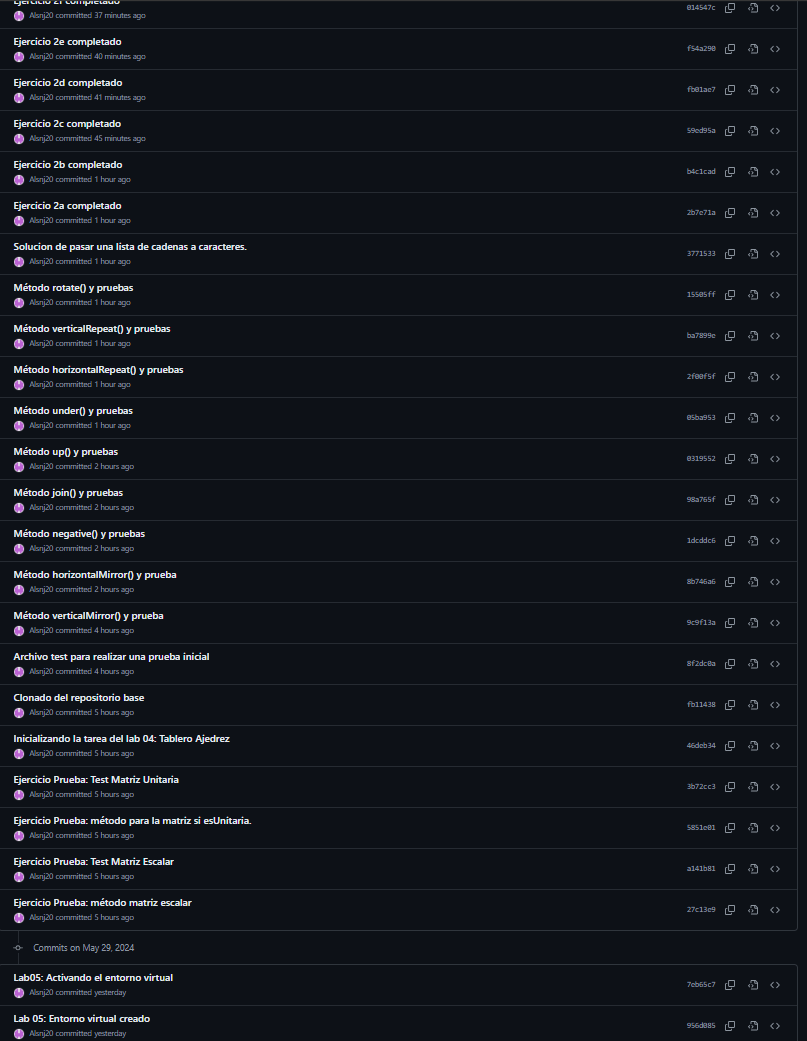
\includegraphics[width=0.9\textwidth,keepaspectratio]{img/commits.png}
	\caption{Lista de commits.}
\end{figure}
\pagebreak
\section{Equipos y materiales utilizados}
\begin{itemize}
	%%%%%%%%%%%%%%%%%%%%%%%%%%%%%%%%%%%%%%%%%%%%%%%%%%%%%%%%%%%%%%%%%%%%%%
	\item Cuenta en GitHub con el correo institucional.
	\item Sistema Operativo Microsoft Windows 10
	\item Visual Studio Code
	\item Git
	\item Windows PowerShell
	\item Python
	\item Navegador Mozilla Firefox
	      %%%%%%%%%%%%%%%%%%%%%%%%%%%%%%%%%%%%%%%%%%%%%%%%%%%%%%%%%%%%%%%%%%%%%%
\end{itemize}
\pagebreak

\section{Solución}
\begin{itemize}
	\item La solución de la tarea se encuentra en el directorio Tarea-del-Ajedrez, instalar primero las dependencias necesarias con el siguiente comando:
	\item Instalar pygame
	\begin{figure}[H]
		\centering
		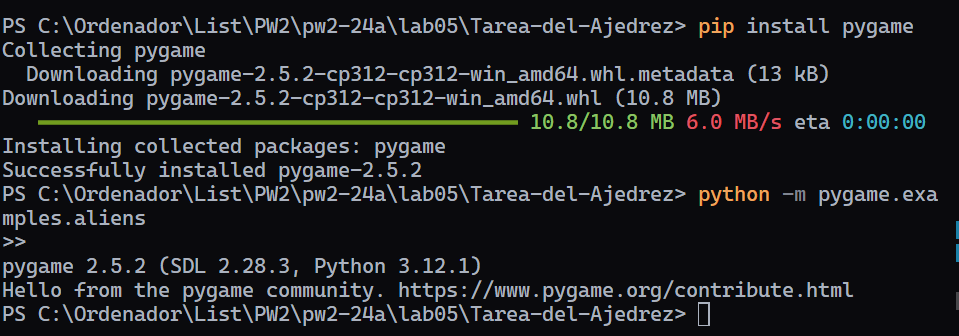
\includegraphics[height=0.3\textwidth]{img/pygame.png}
		\caption{Instalar pygame}
	\end{figure}
	\item Trabajaremos con la clase Picture y ejecutaremos a traves de draw.py
	\begin{figure}[H]
		\centering
		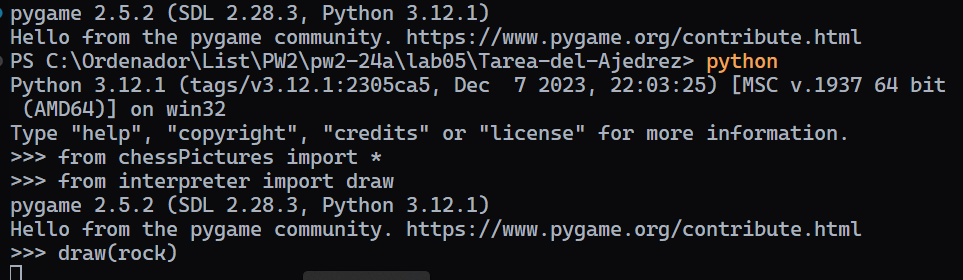
\includegraphics[height=0.25\textwidth]{img/draw.png}
		\caption{Ejecutar draw.py}
	\end{figure}
	\item Prueba de ejecución
	\begin{figure}[H]
		\centering
		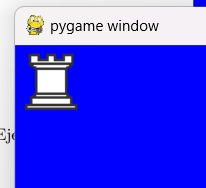
\includegraphics[height=0.3\textwidth]{img/drawPrueba.png}
		\caption{Prueba de ejecución}
	\end{figure}
\end{itemize}
\subsection{Código}
\begin{block}
	\inputminted{python}{../Tarea-del-Ajedrez/picture.py}
	\caption{picture.py}
\end{block}
\subsubsection{Funcionalidad}
\begin{itemize}
	\item {\textbf{init(self, img):}  Este es el constructor de la clase. Inicializa una nueva instancia de Picture con una imagen img, que parece ser una lista de cadenas.}
	\item {\textbf{eq(self, other):}  Este método comprueba si dos instancias de Picture son iguales comparando sus imágenes.}
	\item {\textbf{invColor(self, color):} Este método privado invierte un color si el color está en el diccionario inverter importado del módulo colors.}
	\item {\textbf{verticalMirror(self):} Este método crea una nueva imagen que es un reflejo vertical de la imagen original. Esto se logra invirtiendo el orden de las filas en img(arreglo de strings).}
	\item {\textbf{horizontalMirror(self):} Este método crea una nueva imagen que es un reflejo horizontal de la imagen original. Esto se logra invirtiendo el orden de los caracteres en cada fila de img.}
	\item {\textbf{negative(self):} Este método crea una nueva imagen que es el negativo de la imagen original. Esto se logra invirtiendo los colores de cada pixel en img.}
	\item {\textbf{join(self, other):} Este método crea una nueva imagen que es la imagen original con la imagen other a su derecha. Esto se logra concatenando las filas de img con las filas de other.img.}
	\item {\textbf{up(self, other):} Este método crea una nueva imagen que es la imagen original con la imagen other encima de ella. Esto se logra concatenando las filas de other.img con las filas de img.}
	\item {\textbf{under(self, other):} Este método crea una nueva imagen que es la imagen original con la imagen other debajo de ella. Esto se logra concatenando las filas de img con las filas de other.img.}
	\item {\textbf{horizontalRepeat(self, n):} Este método crea una nueva imagen que es la imagen original repetida n veces a su derecha. Esto se logra concatenando las filas de img con las filas de img n veces.}
	\item {\textbf{verticalRepeat(self, n):} Este método crea una nueva imagen que es la imagen original repetida n veces debajo de ella. Esto se logra concatenando las filas de img con las filas de img n veces.}
\end{itemize}

\subsection{Ejercicios}
\subsubsection{Ejercicio 2a}
\begin{block}
	\inputminted{python}{../Tarea-del-Ajedrez/Ejercicio2a.py}
	\begin{figure}[H]
		\centering
		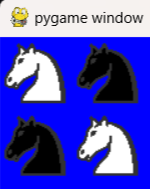
\includegraphics[height=0.3\textwidth]{img/2a.png}
		\caption{Ejercicio2a.py}
	\end{figure}
\end{block}
\subsubsection{Ejercicio 2b}
\begin{block}
	\inputminted{python}{../Tarea-del-Ajedrez/Ejercicio2b.py}
	\begin{figure}[H]
		\centering
		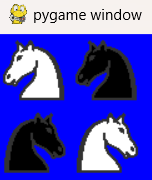
\includegraphics[height=0.3\textwidth]{img/2b.png}
		\caption{Ejercicio2b.py}
	\end{figure}
\end{block}
\pagebreak
\subsubsection{Ejercicio 2c}
\begin{block}
	\inputminted{python}{../Tarea-del-Ajedrez/Ejercicio2c.py}
	\begin{figure}[H]
		\centering
		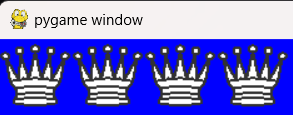
\includegraphics[height=0.2\textwidth]{img/2c.png}
		\caption{Ejercicio2c.py}
	\end{figure}
\end{block}
\subsubsection{Ejercicio 2d}
\begin{block}
	\inputminted{python}{../Tarea-del-Ajedrez/Ejercicio2d.py}
	\begin{figure}[H]
		\centering
		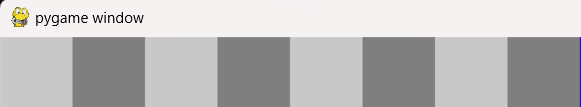
\includegraphics[height=0.1\textwidth]{img/2d.png}
		\caption{Ejercicio2d.py}
	\end{figure}
\end{block}
\subsubsection{Ejercicio 2e}
\begin{block}
	\inputminted{python}{../Tarea-del-Ajedrez/Ejercicio2e.py}
	\begin{figure}[H]
		\centering
		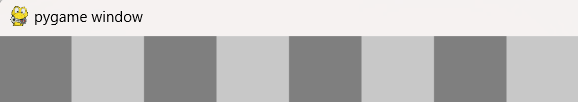
\includegraphics[height=0.1\textwidth]{img/2e.png}
		\caption{Ejercicio2e.py}
	\end{figure}
\end{block}
\subsubsection{Ejercicio 2f}
\begin{block}
	\inputminted{python}{../Tarea-del-Ajedrez/Ejercicio2f.py}
	\begin{figure}[H]
		\centering
		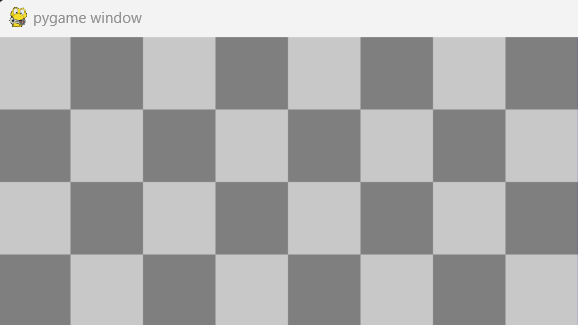
\includegraphics[height=0.5\textwidth]{img/2f.png}
		\caption{Ejercicio2f.py}
	\end{figure}
\end{block}
\subsubsection{Ejercicio 2g}
\begin{block}
	\inputminted{python}{../Tarea-del-Ajedrez/Ejercicio2g.py}
	\begin{figure}[H]
		\centering
		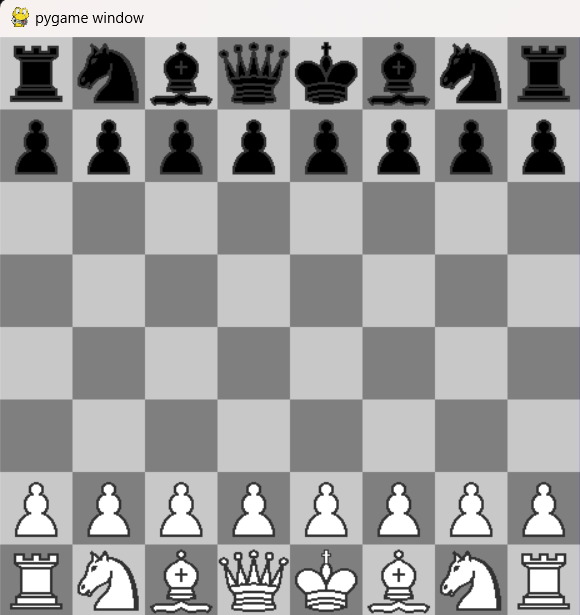
\includegraphics[height=0.6\textwidth]{img/2g.png}
		\caption{Ejercicio2g.py}
	\end{figure}
\end{block}
\section{URL del repositorio en GitHub}
\begin{itemize}
	\item \url{https://github.com/Alsnj20/pw2-24a/tree/main/lab05}
\end{itemize}
\pagebreak
\section{Estructura de laboratorio \itemPracticeNumber}
\begin{itemize}
	\item El contenido que se entrega en este laboratorio es el siguiente:
\end{itemize}
\begin{lstlisting}{language=bash}
lab05/
  |---/execises
      |---/_pycache_
      |---esEscalar.py
      |---esUnitaria.py
      |---test_esEscalar.py
      |---test_esUnitaria.py
  |---/latex
      |--- linopinto_pw2_24a_lab05.tex
      |--- linopinto_pw2_24a_lab05.pdf
			|---/img
					|---2a.png
					|---2b.png
					|---2c.png
					|---2d.png
					|---2e.png
					|---2f.png
					|---2g.png
					|---commits.png
					|---draw.png
					|---drawPrueba.png
					|---episunsa.png
					|---logo_abet.png
					|---pygame.png
	|---/my_env
	|---/Tarea1-del-Ajedrez
			|---/__pycache__
			|---.gitignore
			|---chessPicture.py
			|---colors.py
			|---Ejercicio2a.py
			|---Ejercicio2b.py
			|---Ejercicio2c.py
			|---Ejercicio2d.py
			|---Ejercicio2e.py
			|---Ejercicio2f.py
			|---Ejercicio2g.py
			|---interpreter.py
			|---picture.py
			|---pieces.py
			|---test.py
  |--- README.md
  |---.gitignore
\end{lstlisting}

\pagebreak
\section{Rúbrica}

\begin{table}[H]
	\centering
	\caption{Tabla: Rúbrica para contenido del Informe y evidencias}
	\begin{tabular}{|p{2cm}|p{6cm}|c|c|c|c|}
			\hline
			\multicolumn{2}{|c|}{\textbf{Contenido y demostración}} & \textbf{Puntos} & \textbf{Checklist} & \textbf{Estudiante} & \textbf{Profesor} \\ \hline
			1. GitHub & Repositorio se pudo clonar y se evidencia la estructura adecuada para revisar los entregables. (Se descontará puntos por error o observación) & 4 & × & 4 & \\ \hline
			2. Commits & Hay porciones de código fuente asociado a los commits planificados con explicaciones detalladas. (El profesor puede preguntar para refrendar calificación) & 4 & × & 4 & \\ \hline
			3. Ejecución & Se incluyen comandos para ejecuciones y pruebas del código fuente explicadas gradualmente que permitirían replicar el proyecto. (Se descontará puntos por cada omisión) & 4 & ×  & 4 & \\ \hline
			4. Pregunta & Se responde con completitud a la pregunta formulada en la tarea. (El profesor puede preguntar para refrendar calificación) & 2 & × & 2 & \\ \hline
			7.Ortografía & El documento no muestra errores ortográficos. (Se descontará puntos por error encontrado) & 2 & × & 1 & \\ \hline
			8. Madurez & El Informe muestra de manera general una evolución de la madurez del código fuente con explicaciones puntuales pero precisas, agregando diagramas generados a partir del código fuente y refleja un acabado impecable. (El profesor puede preguntar para refrendar calificación) & 4 & × & 4 & \\ \hline
			\multicolumn{2}{|c|}{\textbf{Total}} & 20 & Completo & 19 & \\ \hline
	\end{tabular}
\end{table}

\section{Referencias}
\begin{itemize}
	\item \url{https://github.com/}
	\item \url{https://git-scm.com/}
	\item \url{https://www.w3schools.com/python/}
\end{itemize}

\pagebreak
\bibliographystyle{apalike}
\bibliographystyle{IEEEtranN}
\bibliography{bibliography}

\end{document}